\chapter{Проверка на однородность}\label{cha:uniform}

Используется только для непрерывных распределений.\\

\section{Сравнение двух выборок}\label{cha:uniform/sec:2}

Пусть $X = (X_1, \dots, X_n)$ имеет распределение $F$, $Y = (Y_1, \dots, Y_n)$ имеет распределение $G$. $X$ и $Y$ - две независимые выборки.\\
$H_0: F = G$.

	\subsection{Критерий Смирного}\label{cha:uniform/sec:2/smirn}

		\subsubsection*{Теория}\label{cha:uniform/sec:2/subsec:smirn/subsubsec:theory}

		Является непараметрическим критерием.

		$$T = \sqrt{\frac{n m }{n+m}}\cdot \underset{x \in \mathbb{R}}{sup} \; |\hat{F_n}(x) - \hat{G_m}(x)|$$
		Асимптотический критерий:
		$$\begin{gathered}
			T \xrightarrow[H_0]{d}\xi, \;\; \xi \text{ имеет распределение Колмогорова} \\
			C_{\text{кр}} = [K_{1-\alpha}, +\infty)
		\end{gathered}$$

		\subsubsection*{Пример}\label{cha:uniform/sec:2/subsec:smirn/subsubsec:prob}

		\begin{lstlisting}[language=Python]
			from scipy.stats import norm, t
			x = norm.rvs(size = 200, loc = 0, scale = 1)
			y = t.rvs(size=300, df = 7)
			z = norm.rvs(size = 400, loc = 0, scale = 3)
			from scipy.stats import ks_2samp
			s_2samp(x, y)
			ks_2samp(x, z)
		\end{lstlisting}

\section{Сравнение $k \ge 2$ выборок}\label{cha:uniform/sec:k}

	\subsection{Общий критерий Андерсона-Дарлинга}\label{cha:uniform/sec:k/andersdarling}

		\subsubsection*{Теория}\label{cha:uniform/sec:k/subsec:andersdarling/subsubsec:theory}

		Является непараметрическим критерием.\\

		Имеем $k \ge 2$ независимых выборок. $(X_{11}, \dots, X_{1 n_1})$ имеет распределение $F_1$, $\dots$, $(X_{k1}, \dots, X_{k n_k})$ имеет распределение $F_k$. $H_0: F_1 = \dots = F_k$. $\hat{F_1}, \dots, \hat{F_k}$ - ЭФР, $N = n_1 + \dots + n_k$. $\hat{H_N}(x)$ -- ЭФР по всей совокупности из $N$ наблюдений.
		$$\Omega^2 = \underset{i=1}{\overset{k}{\sum}}n_i \cdot \underset{\mathbb{R}}{\overset{}{\int}}\frac{\left( \hat{F_i}(x) - \hat{H_N}(x) \right)^2}{\hat{H_N}(x) (1 - \hat{H_N}(x))} d \hat{H_N}(x)$$ 

		\subsubsection*{Пример}\label{cha:uniform/sec:k/subsec:andersdarling/subsubsec:prob}

		В качестве результата тест выдает значение статистики, набор квантилей $x_{1-\alpha}$ для значений $\alpha$ вида 25$\%$, 10$\%$, 5$\%$, 2.5$\%$, 1$\%$, 0.5$\%$, 0.1$\%$ и p-value.

		\begin{lstlisting}[language=Python]
			from scipy.stats import anderson_ksamp
			anderson_ksamp([x, y])
		\end{lstlisting}

	\subsection{Критерий Краскела-Уоллиса}\label{cha:uniform/sec:k/kraskel}

		\subsubsection*{Теория}\label{cha:uniform/sec:k/subsec:kraskel/subsubsec:theory}

		Применяется в непараметрическом случае (хотя бы одна выборка ненормальна).\\

		Имеем $k \ge 2$ выборок:
		$$\begin{pmatrix}
			X_{11} \\ \vdots \\ X_{n_1 1}
		\end{pmatrix}, \begin{pmatrix}
			X_{12} \\ \vdots \\ X_{n_2 2}
		\end{pmatrix}, \dots, \begin{pmatrix}
			X_{1k} \\ \vdots \\ X_{n_k k}
		\end{pmatrix}$$

		Для элемента $X_{ij}$ $i$ - это номер элемента в $j$-ой выборке, а $j$ - это номер выборки. $N = \underset{j=1}{\overset{k}{\sum}}n_j$.\\

		$X_{ij} = \mu + \beta_j + \varepsilon_{ij}$, где $\beta_j$ - эффект от воздействия фактора, $\varepsilon_{ij}$ - случайные ошибки. Необходимо, чтобы были выполнены следующие условия:
		\begin{itemize}
			\item[$\bullet$] все $\varepsilon_{ij}$ независимы
			\item[$\bullet$] все $\varepsilon_{ij}$ имеют одинаковое непрерывное распределение
		\end{itemize}
		$H_0: \beta_1 = \dots = \beta_k$. $H_1:$ не все $\beta_j$ равны. Строим статистику: смешиваем все $N$ наблюдений, $R_{ij}$ - ранг $X_{ij}$, $S_j = \underset{i=1}{\overset{n_j}{\sum}}R_{ij}$ - сумма рангов $j$-ой выборки, $R_{\cdot j} = \frac{S_j}{n_j}$ - средний ранг $j$-ой выборки, $R_{\cdot \cdot} = \frac{1}{N}\underset{i,j}{\overset{}{\sum}}R_{ij} = \frac{N+1}{2}$ - общий средний ранг.
		$$\begin{gathered}
			H = \frac{12}{N(N+1)}\cdot \underset{j=1}{\overset{k}{\sum}}n_j (R_{\cdot j} - R_{\cdot \cdot})^2 = \left[ \frac{12}{N (N+1)} \cdot \underset{j=1}{\overset{k}{\sum}}\frac{S_j^2}{n_j} \right] - 3 (N+1) \\
			H \xrightarrow[H_0]{} \text{ табличное распределение}\\
			C_{\text{кр}} = [h_{1-\alpha}, +\infty)
		\end{gathered}$$
		Асимптотический критерий:
		$$H \xrightarrow[H_0]{d}\chi^2 (k-1), \; \; C_{\text{кр}} = [ \chi_{1-\alpha}^2 (k-1), +\infty)$$

		\subsubsection*{Пример}\label{cha:uniform/sec:k/subsec:kraskel/subsubsec:prob}

		\begin{problem}
			В файле «Harvest.txt» представлены данные об урожае клубники (в квартах) с участков трех типов почв. Влияет ли (на уровне значимости 5$\%$) тип почвы на урожайность?
		\end{problem}
		\begin{solution}
			\begin{lstlisting}[language=Python]
				data = pd.read_csv("Harvest.txt")
				x = data['x']
				y = data['y']
				z = data['z']
				st.shapiro(x)
				st.shapiro(y)
				st.shapiro(z)
				from scipy.stats import kruskal
				kruskal (x, y, z)
			\end{lstlisting}
		\end{solution}

	\subsection{Критерий Джонкхиера}\label{cha:uniform/sec:k/john}

		\subsubsection*{Теория}\label{cha:uniform/sec:k/subsec:john/subsubsec:theory}

		$H_0: \beta_1 = \dots = \beta_k$, $H_1: \beta_1 \le \beta_2 \le \dots \le \beta_k$ - альтернатива возрастания влияния фактора. Данный тест имеет большую мощность при такой альтернативе, чем тест Краскела-Уоллеса.\\

		Статистика: $C_k^2 = \frac{k(k-1)}{2}$ - кол-во пар выборок. Считает $\frac{k(k-1)}{2}$ значений статистики Манна-Уитни.
		$$\begin{gathered}
			U_{rs} = \underset{i=1}{\overset{n_r}{\sum}}\underset{j=1}{\overset{n_s}{\sum}}\mathbb{I}(X_{i r} < X_{j s}), \;\; 1 \le r \le s \le k \\
			J = \underset{r < s}{\overset{}{\sum}}U_{rs} = \underset{r=1}{\overset{k-1}{\sum}}\underset{s=r+1}{\overset{k}{\sum}}U_{rs} \text{ -- имеет табличное распределение}\\
			C_{\text{кр}} = [j_{1-\alpha}, +\infty)
		\end{gathered}$$
		Асимптотический критерий:
		$$\begin{gathered}
			J^{*} = \frac{J - E J}{\sqrt{D J}} \xrightarrow[H_0]{d}N(0,1) \\
			H_0 \; \Rightarrow \; \begin{cases}
				E J = \frac{1}{4}\left( N^2 - \underset{j=1}{\overset{k}{\sum}}n_j^2 \right) \\
				D J = \frac{1}{72} \left( N^2 (2N +3) - \underset{j=1}{\overset{k}{\sum}}n_j^2 (2n_j + 3) \right)
			\end{cases}
		\end{gathered}$$

		\subsubsection*{Пример}\label{cha:uniform/sec:k/subsec:john/subsubsec:prob}

		надо реализовать

	\subsection{Критерий Неменьи}\label{cha:uniform/sec:k/nemeni}

		\subsubsection*{Теория}\label{cha:uniform/sec:k/subsec:nemeni/subsubsec:theory}

		Nemenyi test принадлежит семейству Post Hoc tests - они мощнее, чем попарный t-test, а также легки в подсчете.\\

		$H_0: \beta_r = \beta_s$, $H_1: \beta_r \not = \beta_s$.
		$$\begin{gathered}
			T = \frac{R_{\cdot r} - R_{\cdot s}}{\sqrt{\frac{N(N+1)}{24}\left( \frac{1}{n_r} + \frac{1}{n_s} \right)}} \sim \text{ табличное распределение} \\
			|T| > q_{\text{crit}} \; \Rightarrow \; \text{отвергаем } H_0
		\end{gathered}$$

		Желательно делать поправку на множественное сравнение.

		\subsubsection*{Пример}\label{cha:uniform/sec:k/subsec:nemeni/subsubsec:prob}

		\begin{lstlisting}[language=Python]
			import scikit_posthocs as sp
			sp.posthoc_nemenyi([x, y, z])
			nem_res = sp.posthoc_nemenyi([x, y, z])
			nem_res[1][2]
		\end{lstlisting}

	\subsection{Критерий Бартлетта}\label{cha:uniform/sec:k/bartlet}

		\subsubsection*{Теория}\label{cha:uniform/sec:k/subsec:bartlet/subsubsec:theory}

		Применяется в предположении, что $X_{ij}\sim N (\mu_j, \sigma_j^2)$, параметры распределения неизвестны. Критерий применяется для получения информации про дисперсию.\\

		$H_0: \sigma_1 = \dots = \sigma_k$, $H_1:$ не все $\sigma_j$ равны. Статистика:
		$$\begin{gathered}
			B^{*} = \gamma^{-1} \cdot N \cdot \ln B, \text{ где}\\
			\;\;\;\; \gamma = 1 + \frac{1}{3(k-1)} \left[ \underset{j=1}{\overset{k}{\sum}}\frac{1}{n_j} - \frac{1}{N} \right] \\
			B = \frac{\left( \frac{1}{N} \underset{j=1}{\overset{k}{\sum}}n_j S_j^2 \right)}{\sqrt[N]{\underset{j=1}{\overset{k}{\Pi}} (S_j^2)^{n_j}}} \\
			S_j^2 = \frac{1}{n_j - 1} \underset{i=1}{\overset{n_j}{\sum}}(X_{ij} - X_{\cdot j})^2
		\end{gathered}$$
		При $n_j \ge 3$ $B^{*} \Hosim \chi^2 (k-1)$.\\

		При отвержении $H_0$ возникает проблема множественных сравнений, поэтому необходимо делать \blue{поправку Бонферонни}: $\alpha \to \frac{\alpha}{C_k^2} = \tilde{\alpha}$.

		\subsubsection*{Пример}\label{cha:uniform/sec:k/subsec:bartlet/subsubsec:prob}

		\begin{lstlisting}[language=Python]
			from scipy.stats import bartlett
			bartlett(x, y, z)
		\end{lstlisting}

	\subsection{Критерий Данна}\label{cha:uniform/sec:k/dann}

		\subsubsection*{Теория}\label{cha:uniform/sec:k/subsec:dann/subsubsec:theory}

		Является непараметрическим тестом, применяется для больших выборок, т.е. является асимптотическим.\\

		$H_0: \beta_r = \beta_s$, $H_1: \beta_r \not = \beta_s$.
		$$T = \frac{R_{\cdot r} - R_{\cdot s}}{\sqrt{\frac{N(N+1)}{12}\left( \frac{1}{n_r} + \frac{1}{n_s} \right)}}$$

		\begin{center}
			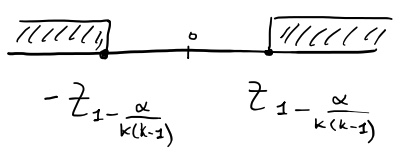
\includegraphics[scale=0.6]{uniform1}
		\end{center}

		$$1 - \frac{\alpha}{2} \to 1 - \frac{\alpha}{C_k^2 \cdot 2} = 1 - \frac{\alpha}{k (k-1)}$$

		\subsubsection*{Пример}\label{cha:uniform/sec:k/subsec:dann/subsubsec:prob}

		\begin{lstlisting}[language=Python]
			sp.posthoc_dunn([x, y, z], p_adjust = 'bonferroni')
			dunn_res = sp.posthoc_dunn([x, y, z], p_adjust = 'bonferroni')
			dunn_res[1][3]
			dunn_res = sp.posthoc_dunn([x, y, z], p_adjust = None)
			dunn_res[1][3]*3
		\end{lstlisting}

	\subsection{ANOVA}\label{cha:uniform/sec:k/anova}

		\subsubsection*{Теория}\label{cha:uniform/sec:k/subsec:anova/subsubsec:theory}

		Применяется в случае $k$ нормальных выборок - однофакторный дисперсионный анализ: ANOVA = Analysis of Variance. \\

		$X_{ij} \sim N(\mu_j, \sigma^2)$. Для применения необходимо выполнния следующих условий:
		\begin{itemize}
			\item[$\bullet$] нормальное распределение всех выборок
			\item[$\bullet$] равенство дисперсий всех выборок
			\item[$\bullet$] независимость наблюдений
		\end{itemize}

		$H_0: \mu_1 = \dots = \mu_k$, $H_1:$ не все $\mu_j$ равны. Строим статистику:
		$$\begin{gathered}
			X_{\cdot j} = \frac{1}{n_j}\underset{i=1}{\overset{n_j}{\sum}}X_{ij} = \overline{X_j} \text{ - среднее } j\text{-ой выборки}\\
			X_{\cdot \cdot} = \frac{1}{N} \underset{j=1}{\overset{k}{\sum}}\underset{i=1}{\overset{n_j}{\sum}}X_{ij}\\
			F = \frac{N-k}{k-1}\cdot \frac{\underset{j=1}{\overset{k}{\sum}}n_j (X_{\cdot j} - X_{\cdot \cdot})^2}{\underset{j=1}{\overset{k}{\sum}}\underset{i=1}{\overset{n_j}{\sum}}(X_{ij} - X_{\cdot j})^2} \Hosim F(k-1, N-k)
		\end{gathered}$$

		Если $n_1 = \dots = n_k$, то при небольшом отклонении от нормальности распределений и от равенства дисперсий ANOVA все равно можно применять.

		\subsubsection*{Пример}\label{cha:uniform/sec:k/subsec:anova/subsubsec:prob}

		\begin{lstlisting}[language=Python]
			from scipy.stats import f_oneway
			f_oneway(x, y, z)
		\end{lstlisting}

	\subsection{LSD Фишера}\label{cha:uniform/sec:k/lsd}

		\subsubsection*{Теория}\label{cha:uniform/sec:k/subsec:lsd/subsubsec:theory}

		Fisher's least significant difference test применяется в предположении нормальности данных. $X_{ij} \sim N(\mu_j, \sigma^2)$. Дисперсии равны, выборки независимы.\\

		$H_0: \mu_r = \mu_s$, $H_1: \mu_r \not = \mu_s$.
		$$\begin{gathered}
			T = \frac{X_{\cdot r} - X_{\cdot s}}{\sqrt{MS_E \left( \frac{1}{n_r} + \frac{1}{n_s} \right)}} \Hosim t (N-k), \text{ где}\\
			X_{\cdot r} = \frac{1}{n_r} \underset{i=1}{\overset{n_r}{\sum}}X_{ir}, \; MS_E = \frac{SS_E}{N_k}, \; SS_E = \underset{j=1}{\overset{k}{\sum}}\underset{i=1}{\overset{n_j}{\sum}}(X_{ij} - X_{\cdot j})^2 = \underset{j=1}{\overset{k}{\sum}}(n_j - 1)S_j^2
		\end{gathered}$$

		\subsubsection*{Пример}\label{cha:uniform/sec:k/subsec:lsd/subsubsec:prob}

		\begin{lstlisting}[language=Python]
			def LSD_Fisher(i, j, samples):
			    n1, n2 = len(samples[i]), len(samples[j])
			    k = len(samples)
			    N = np.sum([len(samples[l]) for l in range(k)])
			    SSe = np.sum([np.var(samples[l], ddof=0) * len(samples[l]) for l in range(k)])
			    stat = (np.mean(samples[i]) - np.mean(samples[j]))/np.sqrt(SSe / (N - k) * (1.0/n1 + 1.0/n2))
			    return 2*np.min([ st.t.cdf(stat, N - k), 1 - st.t.cdf(stat, N - k)])

			LSD_Fisher(0, 2, [x,y,z])
		\end{lstlisting}

	\subsection{Критерий Шеффе}\label{cha:uniform/sec:k/scheffe}

		\subsubsection*{Теория}\label{cha:uniform/sec:k/subsec:scheffe/subsubsec:theory}

		Scheffe's test применяется в предположении нормальности данных.\\

		$X_{ij} \sim N(\mu_j, \sigma^2)$. $H_0: \underset{j=1}{\overset{k}{\sum}}c_j \mu_j = 0$, где $\underset{j=1}{\overset{k}{\sum}}c_j = 0$. $H_1: \underset{j=1}{\overset{k}{\sum}}c_j \mu_j \not = 0$.
		Статистика:
		$$\begin{gathered}
			S = \frac{\left( \underset{j=1}{\overset{k}{\sum}}c_j \cdot X_{\cdot j} \right)^2}{(k-1) MS_E \cdot \underset{j=1}{\overset{k}{\sum}}\frac{c_j^2}{n_j}} \Hosim F(k-1, N-k) \\
			C_{\text{кр}} = [f_{1-\alpha}(k-1, N-k), +\infty)
		\end{gathered}$$

		\subsubsection*{Пример}\label{cha:uniform/sec:k/subsec:scheffe/subsubsec:prob}

		\begin{lstlisting}[language=Python]
			sp.posthoc_scheffe([x, y, z])
			sch_res = sp.posthoc_scheffe([x, y, z])
			sch_res[1][2]
		\end{lstlisting}

\section{Однофакторный дисперсионный анализ для связанных выборок}\label{cha:uniform/sec:anov}

$$\begin{gathered}
	X_{ij} = \mu + \alpha_i + \beta_j + \varepsilon_{ij}\\
	\mu \text{ -- неизвестное среднее, } \varepsilon_{ij} \text{ -- случайные ошибки} \\
	\alpha_i \text{ -- влияние особенностей } i\text{-го объекта}\\
	\beta_j \text{ -- влияние } j\text{-го уровня фактора} 
\end{gathered}$$

Необходимые условия:
\begin{itemize}
	\item[$\bullet$] $\varepsilon_{ij}$ независимы
	\item[$\bullet$] одинаковое непрерывное распределение
\end{itemize}

	\subsection{Критерий Фридмана}\label{cha:uniform/sec:anov/freedman}

		\subsubsection*{Теория}\label{cha:uniform/sec:anov/subsec:freedman/subsubsec:theory}

		Friedman test является непараметрическим тестом.\\

		$H_0: \beta_1 = \dots = \beta_k$, $H_1:$ не все $\beta_j$ равны. Строим статистику: для каждой строки $i$ ранжируем элементы, получаем $R_{ij}$ - ранг $j$-го элемента в $i$-ой строке. $T_j = \underset{i=1}{\overset{n}{\sum}}R_{ij}, \; R_{\cdot j} = \frac{T_j}{n}$.
		$$F = \left[ \frac{12}{nk (k+1)} \cdot \underset{j=1}{\overset{k}{\sum}}T_j^2 \right] - 3n(k+1)$$
		Асимптотический критерий:
		$$F \xrightarrow[H_0]{d}\chi^2 (k-1), \; C_{\text{кр}} = [ \chi_{1-\alpha}^2(k-1), +\infty)$$

		\subsubsection*{Пример}\label{cha:uniform/sec:anov/subsec:freedman/subsubsec:prob}

		\begin{problem}
			Несколько дегустаторов оценивают различные сорта вин. Имеют ли вина значимые отличия на уровне значимости 5$\%$? Данные представлены в файле «Wine.csv».
		\end{problem}
		\begin{solution}
			\begin{lstlisting}[language=Python]
				data = pd.read_csv('Wine.csv', index_col='tasters') 
				data.columns.name = 'wine'
				data_ar = np.array(data)
				data_ar[0]
				data_ar.T[0]
				friedmanchisquare(*data_ar.T) 
			\end{lstlisting}
		\end{solution}

	\subsection{Критерий Пэйджа}\label{cha:uniform/sec:anov/page}

		\subsubsection*{Теория}\label{cha:uniform/sec:anov/subsec:page/subsubsec:theory}

		Page's trend test является непараметрическим тестом.\\

		$H_0: \beta_1 = \dots = \beta_k$, $H_1: \beta_1 \le \beta_2 \le \dots \le \beta_k$.\\

		Статистика: $L = \underset{j=1}{\overset{k}{\sum}}j \cdot T_j = T_1 + 2 T_2 + \dots + k T_k$.
		Асимптотический критерий:
		$$\begin{gathered}
			\frac{L - E L}{\sqrt{D L}} \xrightarrow[H_0]{d}N(0,1), \; C_{\text{кр}} = [Z_{1-\alpha}, +\infty) \\
			H_0 \; \Rightarrow \; \begin{cases}
				E L = \frac{nk (k+1)^2}{4} \\
				D L = \frac{n(k-1)k^2(k+1)^2}{144}
			\end{cases}
		\end{gathered}$$

		\subsubsection*{Пример}\label{cha:uniform/sec:anov/subsec:page/subsubsec:prob}

		\begin{problem}
			Несколько дегустаторов оценивают различные вина, расположенные по увеличению стоимости за бутылку. Имеют ли вина значимые отличия на уровне значимости 5$\%$? Данные представлены в файле «Wine$\_$Page.csv».
		\end{problem}
		\begin{solution}
			\begin{lstlisting}[language=Python]
				data_page = pd.read_csv('Wine_Page.csv', index_col='tasters') 
				data_page.columns.name = 'wine'
				from PageTest import Page
				Page.test(np.array(data_page).tolist(), ascending=True)
			\end{lstlisting}

			Return values:

			L float: Page’s L statistic

			m int: Number of replications (по строкам)

			n int: Number of treatments (по столбцам)

			p float: P-value
		\end{solution}

	\subsection{ANOVA RM}\label{cha:uniform/sec:anov/anovarm}

		\subsubsection*{Теория}\label{cha:uniform/sec:anov/subsec:anovarm/subsubsec:theory}

		Reapeted measures ANOVA, ANOVA RM, RM ANOVA (ANOVA for correlated samples) применяется в случае нормальный наблюдений, т.е.является параметрическим тестом.\\

		Должно быть выполнено условие сферичности: дисперсия по всех наблюдениях одинаковая. Проверка на сферичность проходит с помощью теста Маухли: смотрим $C_k^2$ разностей столбцов, обнулем построчные влияния $\alpha_i$ и применяем тесты по столбцам.\\

		$H_0: \beta_1 = \dots = \beta_k$, $H_1:$ не все $\beta_j$ равны. 
		$$\begin{gathered}
			F = \frac{\left[ \frac{n}{k-1} \cdot \underset{j=1}{\overset{k}{\sum}}(X_{\cdot j} - X_{\cdot \cdot})^2 \right]}{\left[ \frac{1}{(n-1)(k-1)} \cdot \underset{i=1}{\overset{n}{\sum}}\underset{j=1}{\overset{k}{\sum}}(X_{ij} - X_{i \cdot} - X_{\cdot j} + X_{\cdot \cdot})^2 \right]} \\
			X_{i \cdot} = \frac{1}{k} \underset{j=1}{\overset{k}{\sum}}X_{ij}, \; X_{\cdot j} = \frac{1}{n} \underset{i=1}{\overset{n}{\sum}}X_{ij}, \; X_{\cdot \cdot} = \frac{1}{nk}\underset{i=1}{\overset{n}{\sum}}\underset{j=1}{\overset{k}{\sum}}X_{ij}\\
			F \Hosim F \left( k-1, (n-1)(k-1) \right)\\
			C_{\text{кр}} = [ f_{1-\alpha}\left( k-1, (n-1)(k-1) \right), +\infty)
		\end{gathered}$$

		\subsubsection*{Пример}\label{cha:uniform/sec:anov/subsec:anovarm/subsubsec:prob}

		\begin{problem}
			Несколько дегустаторов оценивают различные сорта вин. Имеют ли вина значимые отличия на уровне значимости 5$\%$? Данные представлены в файле «Wine.csv».
		\end{problem}
		\begin{solution}
			\begin{lstlisting}[language=Python]
				data = pd.read_csv('Wine.csv', index_col='tasters') 
				data.columns.name = 'wine'
				data_ar = np.array(data)
				pg.sphericity(data) 
				spher_res = pg.sphericity(data)
				spher_res[4]
				
				resid = data.add(-data.mean(axis=0), axis='columns').add(-data.mean(axis=1), 
						axis='rows') + data.values.mean()

				#data.add(-data.mean(axis=0), axis='columns')
				#data.add(-data.mean(axis=1), axis='rows')

				st.shapiro(resid)
				data.unstack().head()

				data.unstack().to_frame(name='score').head() 

				data.unstack().to_frame(name='score').reset_index()
				data_anova = data.unstack().to_frame(name='score').reset_index()

				an_rm = AnovaRM(data_anova, depvar='score', subject='tasters', within=['wine'])

				res = an_rm.fit()
				pg.rm_anova(data)

				pg.rm_anova(data=data_anova, dv='score', within='wine',
				 subject='tasters', detailed=False)

				rmanova_res = pg.rm_anova(data)
				rmanova_res['p-unc'][0]
			\end{lstlisting}
		\end{solution}















